%*********************第六章******************
\chapter{总结与展望}
\section{工作总结}
本课题专注于异构计算的研究,无论是在高性能计算领域还是通用计算领域,异构计算都变得越来越重要了。本课题选取的两个应用分别是心脏模拟和深度学习领域比较热门的卷积神经网络应用。下面对这两个应用特点进行概述。

首先是心脏组织模拟应用的特点,归纳如下:

\begin{compactitem}
\item[1.]
主体计算是计算密集型。由于本课题采用的是非常精细的细胞模型,心脏细胞内结构复杂, 含有大量的dyad单元,每个dyad单元内又有100多个通道,因此,心脏细胞内的计算量巨大,属于典型的计算密集型应用。虽然也有部分计算,比如细胞内dyad间电压的扩散过程,这是典型的stencil计算,这部分计算属于访存密集型的,但这部分计算只占细胞内所有计算时间的一小部分。因此,主要的计算类型是密集型计算。

\item[2.]
部分计算是控制语句主导的。对于细胞内的dyad单元的通道状态的模拟,按照直接的方法就是对每个dyad单元单独地进行模拟,每一个dyad单元中的通道状态模拟都涉及到中间计算结果与随机数的比较,比较控制语句在某些体系结构中是非常不高效的,比如在MIC加速器上,比较控制语句性能很差。本课题采用的是二项分布随机采样模拟,这是一个随机采样的过程,对每个dyad的所有通道看作一个整体考虑,大大减少了控制比较语句的执行次数。不过还是无法完全避免所有的控制比较语句,所以这部分计算还是占了一定的开销。

\item[3.]
心脏组织的模拟具有多层并行性。心脏组织模拟应用表现出非常丰富的并行性,对计算的需求非常巨大,需要大规模并行系统才能满足。而心脏组织模拟的计算特点非常适合映射到大规模并行计算系统中,首先心脏组织被划分成规则的网格,每一个网格内的细胞计算由一个计算节点负责;其次,针对有多个加速器构成的异构节点,可以根据异构节点中主机CPU和加速器的计算性能比按比例将网格中的细胞进行划分;对于无论是多核CPU还是众核处理器负责的细胞计算,又可以采用OpenMP对细胞进行并行计算;最后每个小核在对单个细胞进行计算时,可以利用单核的SIMD特性对细胞内dyad单元进行向量化。

\item[4.]
心脏组织模拟如果需要模拟更加复杂的行为时,负载会出现不均衡的问题。如果需要模拟复杂的行为,需要给心脏组织的不同部位进行刺激,有时可能需要在不同的时刻进行刺激。由于刺激的细胞将电压传导到周围的细胞,那些已经被传导的细胞的行为与未被传导的细胞的行为是不同的,在模拟它们时所需计算量是有差异的。模拟的行为越复杂,心脏组织不同部位的模拟所需计算量的差异就越大,负载将变得越来越不均衡。本课题只模拟了简单的行为,因此,负载均衡问题不是特别突出。

\item[5.]
心脏组织模拟通信开销小。在心脏组织模拟应用中,发生在每个细胞内的计算相互独立,细胞间唯一发生联系的是细胞内的电压值,细胞内电压的计算与相邻细胞的电压值相关,因此,每个计算节点负责的网格细胞中处于外围的细胞的电压值都需要与处于相邻的网格外围细胞的电压值进行交换,每次时间迭代各个细胞的电压值都需要更新,因此,每个时间迭代步都涉及到电压值的通信。但相比每次迭代发生的计算量,通信开销所占的比例是相当少的,这也是本课题在大规模节点中能取得很好扩展性的一个重要原因。

\item[6.]
精度敏感型。心脏组织模拟中采用精细的细胞模型,对精度要求极高,其中的变量都采用双精度浮点表示。高精度浮点计算将占用更多的计算资源,需要使用更宽的寄存器,意味着SIMD向量计算单元每次能处理的元素将变少。

\end{compactitem}

深度学习利用大量的训练数据对神经网络进行训练,在某些应用领域表现出了非常好的效果。现在比较流行的神经网络是卷积神经网络,目前各种卷积神经网络的设计表明,网络层次越深,精度越高,但问题就是带来计算量的增加。卷积神经网络涉及的计算与心脏组织模拟中的计算在某些方面具有相似的特点,比如都是计算密集型计算。但也表现出不一样的特点,具体如下:
\begin{compactitem}
\item[1.]核心计算表现为矩阵乘运算。卷积神经网络中的每一层卷积层涉及多个通道的输入以及多个通道的卷积核,卷积核与各个通道做完卷积的结果会归一到一个结果。这种计算特点就是矩阵乘运算的特点,因此,对输入和卷积核组做适当的转换,可以转换成两个输入矩阵,然后进行矩阵乘运算,结果矩阵再变换回原有的存储顺序得到结果输出。矩阵乘为计算密集型,适合在GPU异构加速器上实现,比如针对Nvidia的GPU开发的高效库cublas,也有专门针对卷积层计算的cuDNN库,不过其核心还是矩阵乘运算。

\item[2.]前向计算过程对延迟要求低。神经网络在训练好之后,可以用来推断预测,推断预测只需要运行神经网络的前向过程。大数据环境下,数据中心服务器被用来响应用户的深度学习应用,虽然数据中心服务器计算能力强,但某些复杂的神经网络应用对计算需求相对也大,前向计算过程低延迟要求在数据中心服务器也是存在一定的挑战的。而对于像手机等嵌入式移动终端设备,卷积神经网络前向过程的低延迟实现就更加必需了。无论是针对数据中心还是嵌入式移动终端,对卷积计算进行并行加速都是非常必需的,本课题研究的Winograd算法是对卷积计算的算法改进,目的就是降低矩阵乘运算的数量,从而降低计算量,然而其中引入的变换部分是访存密集型,需要进行适当的访存优化。可以从理论上对Winograd算法进行分析,Winograd算法相比直接的卷积计算能显著减少浮点运算的次数。Winograd算法最后也是转化成矩阵乘运算,只是规模小很多,因此矩阵乘的高效实现库仍然适用,而Winograd算法中的涉及的变换部分也非常适合并行执行,只是这部分对访存带宽要求比较高。针对前行计算过程进行并行加速的另一种方法就是模型并行,这是多设备间的并行,将总计算划分到多个设备上执行,这种方法也能加速前向计算过程,但可能引入通信开销,这将在下一个特点中详细描述。

\item[3.]前向计算过程具有多种并行模式,不同并行模式涉及不同的通信模式。前向计算过程可以采用数据并行和模型并行两种并行方式,数据并行是在多个加速设备上运行同一个神经网络,针对不同的设备给予不同的数据输入,这种并行方式可以很好地提高吞吐量,但不能降低延迟。而模型并行是将卷积网络的卷积层计算划分到多个设备上计算,每次只处理一个数据输入,因此,这种并行方式可以降低延迟。然而模型并行方法引入了一个新的问题,那就是数据通信问题,对于卷积网络的任一卷积层的计算,各个设备在完成各自的任务后,需要对各自的计算结果进行交换,因此,计算设备越多,通信将越复杂。本课腿研究的优化的通信模式采用一种环形的通信结构,最后的通信开销与计算设备的数目无关。

\item[4.]大规模训练具有大规模计算节点的需求。随着训练数据的大量涌现以及神经网络变得更加复杂,简单的单节点服务器在训练方面很难满足需求了,数据中心一般采用大规模节点进行训练,使得训练时间大大降低。

\item[5.]对数值表示的精度要求相对较低。与科学计算应用不同的是,深度学习应用中计算过程的数值精度表示相对没那么高。特别是前向计算过程,直接将训练好的权值转化为16位浮点,对计算结果基本没什么影响。并且越来越多的研究关注使用更少的位数表示神经网络中的输入和权值,有的甚至使用1位来表示,采用更少的位数表示的好处是,一方面可以减少存储,另一方面可以简化计算,比如采用1位表示,其中只涉及异或和移位操作,相比32位浮点计算,这可以大大简化计算。但采用更少的位数表示存在精度不够的问题,这需要在算法设计和网络结构设计方面做出更多的工作进行弥补。

\item[5.]专用硬件加速器实现趋势。神经网络中网络层的类型包含卷积层、全连接层等几种类型,这些网络层计算比较规则,适合硬件加速器实现。已经有专门针对特定网络结构比如Alexnet网络进行加速的FPGA实现,并取得很好的性能。专用硬件加速器实现神经网络的优点就是功耗低,神经网络计算密集型的特点也非常适合在专用硬件加速器上高效实现。
\end{compactitem}

本课题针对这两种应用分别在两种不同的异构平台上进行映射实现。这两种应用分别来自科学计算领域以及人工智能领域,这两种应用表现出不同的特点。本课题通过对应用特点的分析,采用多种并行策略将应用很好地映射到目标体系结构中。也发现在将应用映射到异构体系结构中,异构体系结构可能存在的问题。比如,对于Xeon Phi加速器来说,每个小核的cache容量不足的问题可能增加访存开销,影响计算单元的输入数据的供给,这也给算法的实现带来了一定的挑战性;控制语句在Xeon Phi加速器上效率并不高,因为控制语句导致Xeon Phi加速器上的SIMD实效,除非重新设计算法,使用向量化指令进行手动向量化,这增加了编程的复杂性。对于GPU异构加速器来说,某些应用特征比如分支语句在GPU上也将变得很低效,因为处于同一个块内的线程的分支语句将串行执行。

\section{未来研究方向}
本课题研究还存在不完善的地方,至少可以从以下方向进一步开展研究:
\begin{compactitem}
\item[1.]解决心脏组织复杂模拟中存在的负载不均衡的问题。首先是节点内的负载问题,其次就是节点间的负载平衡问题。静态分配任务的策略不能解决负载不均衡问题,因此,需要设计一个好的动态分配策略,但动态分配策略又可能带来新的问题,通信量将会增加,这都是下一步值得研究的方向。

\item[2.]神经网络在大规模节点环境下训练的通信优化设计。本课题只研究了前向计算过程中多设备并行中通信优化问题,其实神经网络的大规模训练更需要进行通信优化。因此,可以借鉴本课题的通信模式设计,对神经网络的训练过程进行通信优化,从而可以高效地将训练扩展到更大规模的集群环境下。

\item[3.]基于专用硬件加速器的低精度表示的神经网络结构的设计。大数据环境下,新的数据不断地产生,训练无时无刻发生,因此神经网络训练的成本很重要,采用专用硬件FPGA进行训练加速可以很好解决成本问题。设计一种采用尽量少的位数表示的数值进行一些位操作运算的神经网络结构,对FPGA来说,优势会更大。

\end{compactitem}

%\section{估算科大本部树的数目}

%\section{分析推理过程}
%
%据观察,科大本部园区的树主要是两种分布,一是分布在主干道,二是分布在某些特定区域。针对这两种分布,采用不同的方法统计。
%
%首先是主干道上的统计。据观察分布在主干道上的树的间距基本固定,树的间隔(记为$\Delta$)大约5米,见附图1,因此为了统计主干道上的树的数目,只需要测算主干道的长度$L$,(可以在校园绕有树的主干道走一圈,通过手机记步软件统计步数)。则主干道上的树的数目$N_0$:
%\begin{equation}
%N_0 = 2\times\frac{L}{\Delta} 
%\end{equation}
%
%其次,对于特定区域的树的数目统计,比如对于$A_1$区域,采用采样的方法,估算一下$A_1$区域树的平均密度(一平方米内树的数目)$\alpha_1$,然后再计算$A_1$区域的面积$S_1$,对于$A_1$区域的面积的估算,可以采用某些卫星地图软件,比如google Earth,这个app可以对卫星地图中标定的区域面积进行估算,见附图2。则$A_1$区域的树的数目$N_1$可以通过下面公式计算:
%\begin{equation}
%N_1 = \alpha_1 \times S_1
%\end{equation}
%
%这里稍微详细介绍一下通过采样方法计算$A_1$区域树的平均密度$\alpha_1$。从$A_1$区域中选取$p$个不同位置的子区域,子区域面积大小固定为$s$,然后统计各个子区域的树的数目${n_1, n_2, ..., n_p}$,可以计算出各个子区域的密度$\delta_1, \delta_2, ..., \delta_p$ ,
%\begin{equation}
% \delta_i = \frac{n_i}{s}
%\end{equation}
%
%则$A_1$区域树的平均密度$\alpha_1$可以通过以下公式计算:
%\begin{equation}
% \alpha_1 = \frac{\sum_{i=1}^{p}{\delta_i}}{p}
%\end{equation}
%
%采用类似的方法可以估算出其它区域的树的平均密度。
%
%因此,假设有$m$个区域${A_1, A_2, ..., A_m}$,对应的平均密度为${\alpha_1, \alpha_2, ..., \alpha_m}$,各个子域面积为${S_1, S_2, ..., S_m}$,以及各个区域树的数目为${N_1, N_1, ..., N_m}$,所有区域的树的总数为$N$,则:
%\begin{equation}
%N = \sum_{i=1}^{m}{N_i} = \sum_{i=1}^{m}{ \alpha_i \times S_i}
%\end{equation}
%
% 最后总的树数目为M:
%\begin{equation}
%M = N_0 + N=2 \times \frac{L}{\Delta} + \sum_{i=1}^{m}{N_i} = 2 \times \frac{L}{\Delta} + \sum_{i=1}^{m}{ \alpha_i \times S_i}
%\end{equation} 
%
%\section{附}
%
%\begin{figure*}[tbh]%\small
%\centering
%\resizebox{\textwidth}{!}{
%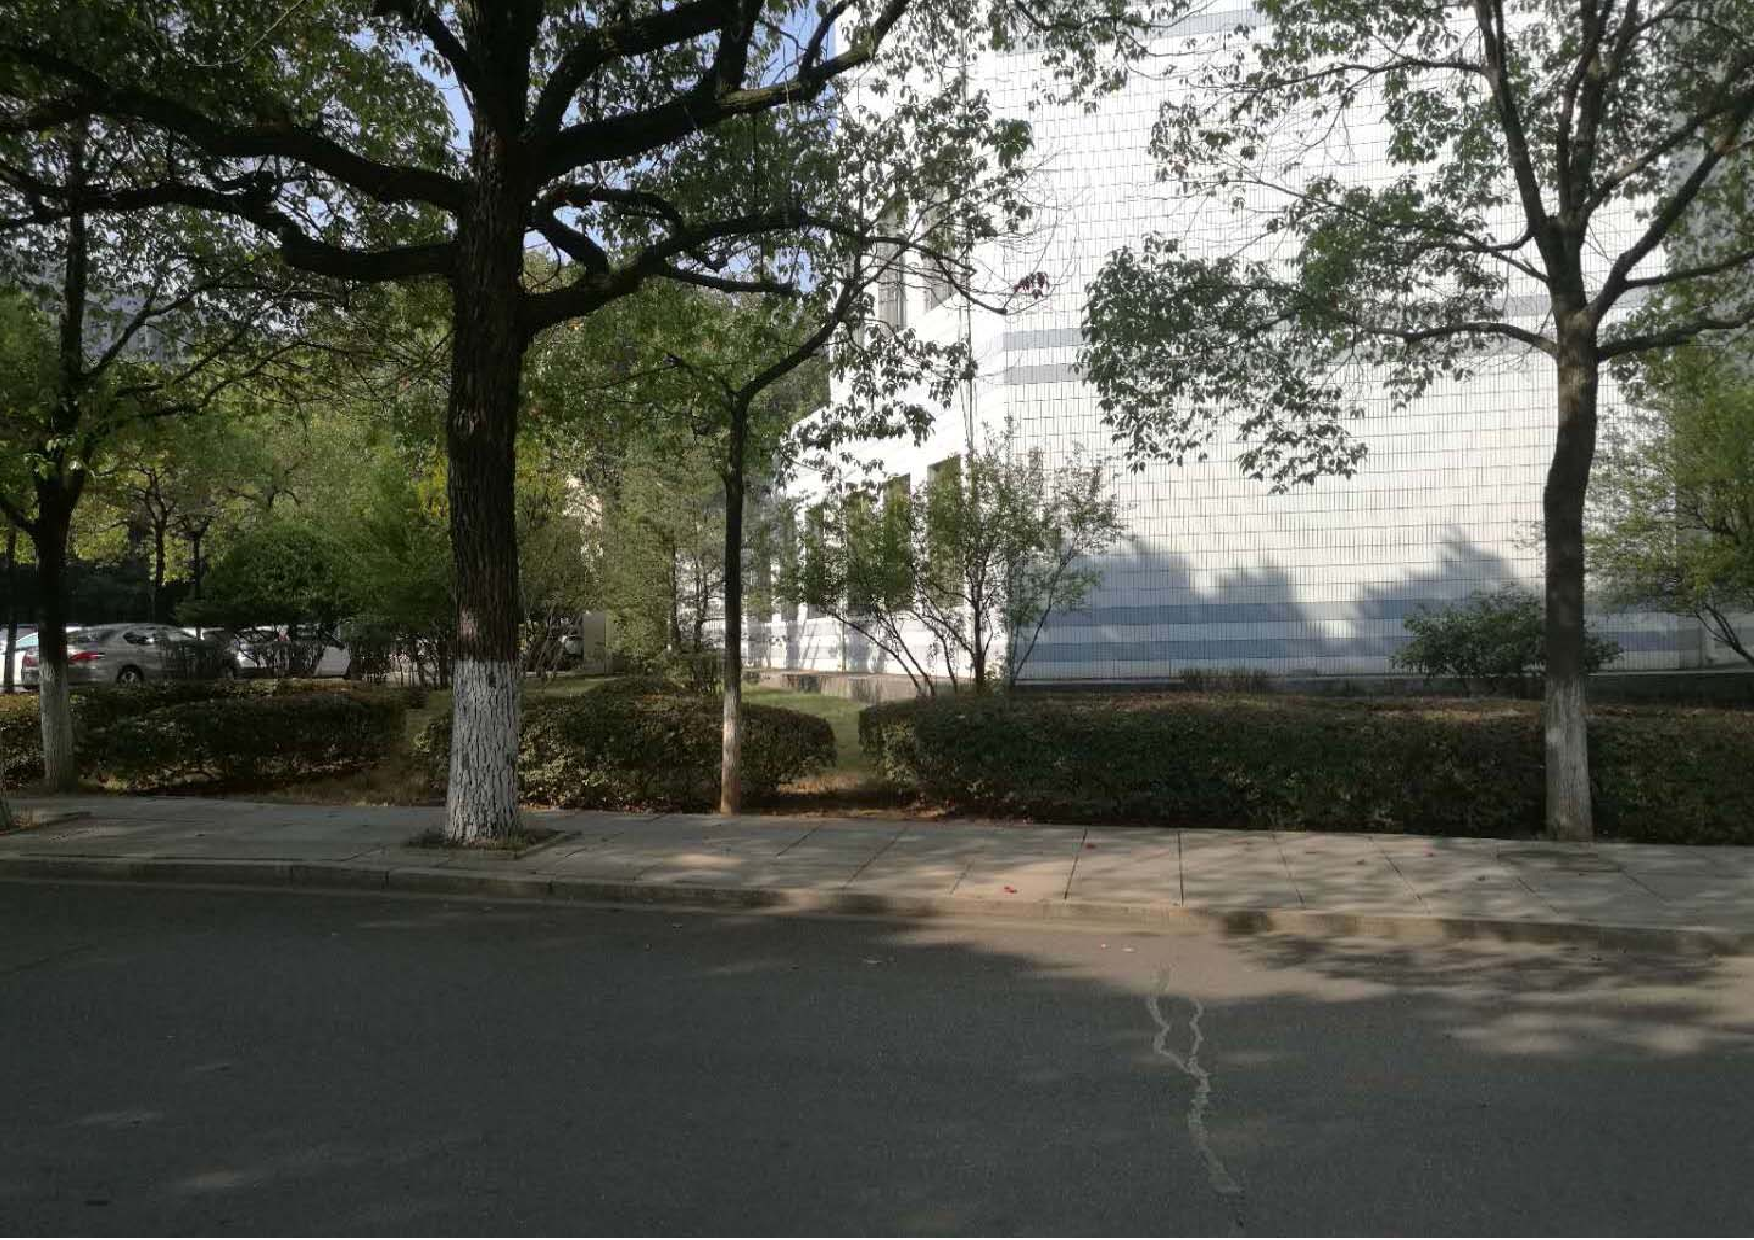
\includegraphics{figs/1.pdf}
%}
%\caption{主干道上树的间距。}
%\label{distance}
%\end{figure*}
%
%\begin{figure*}[tbh]%\small
%\centering
%%\resizebox{\textwidth}{!}{
%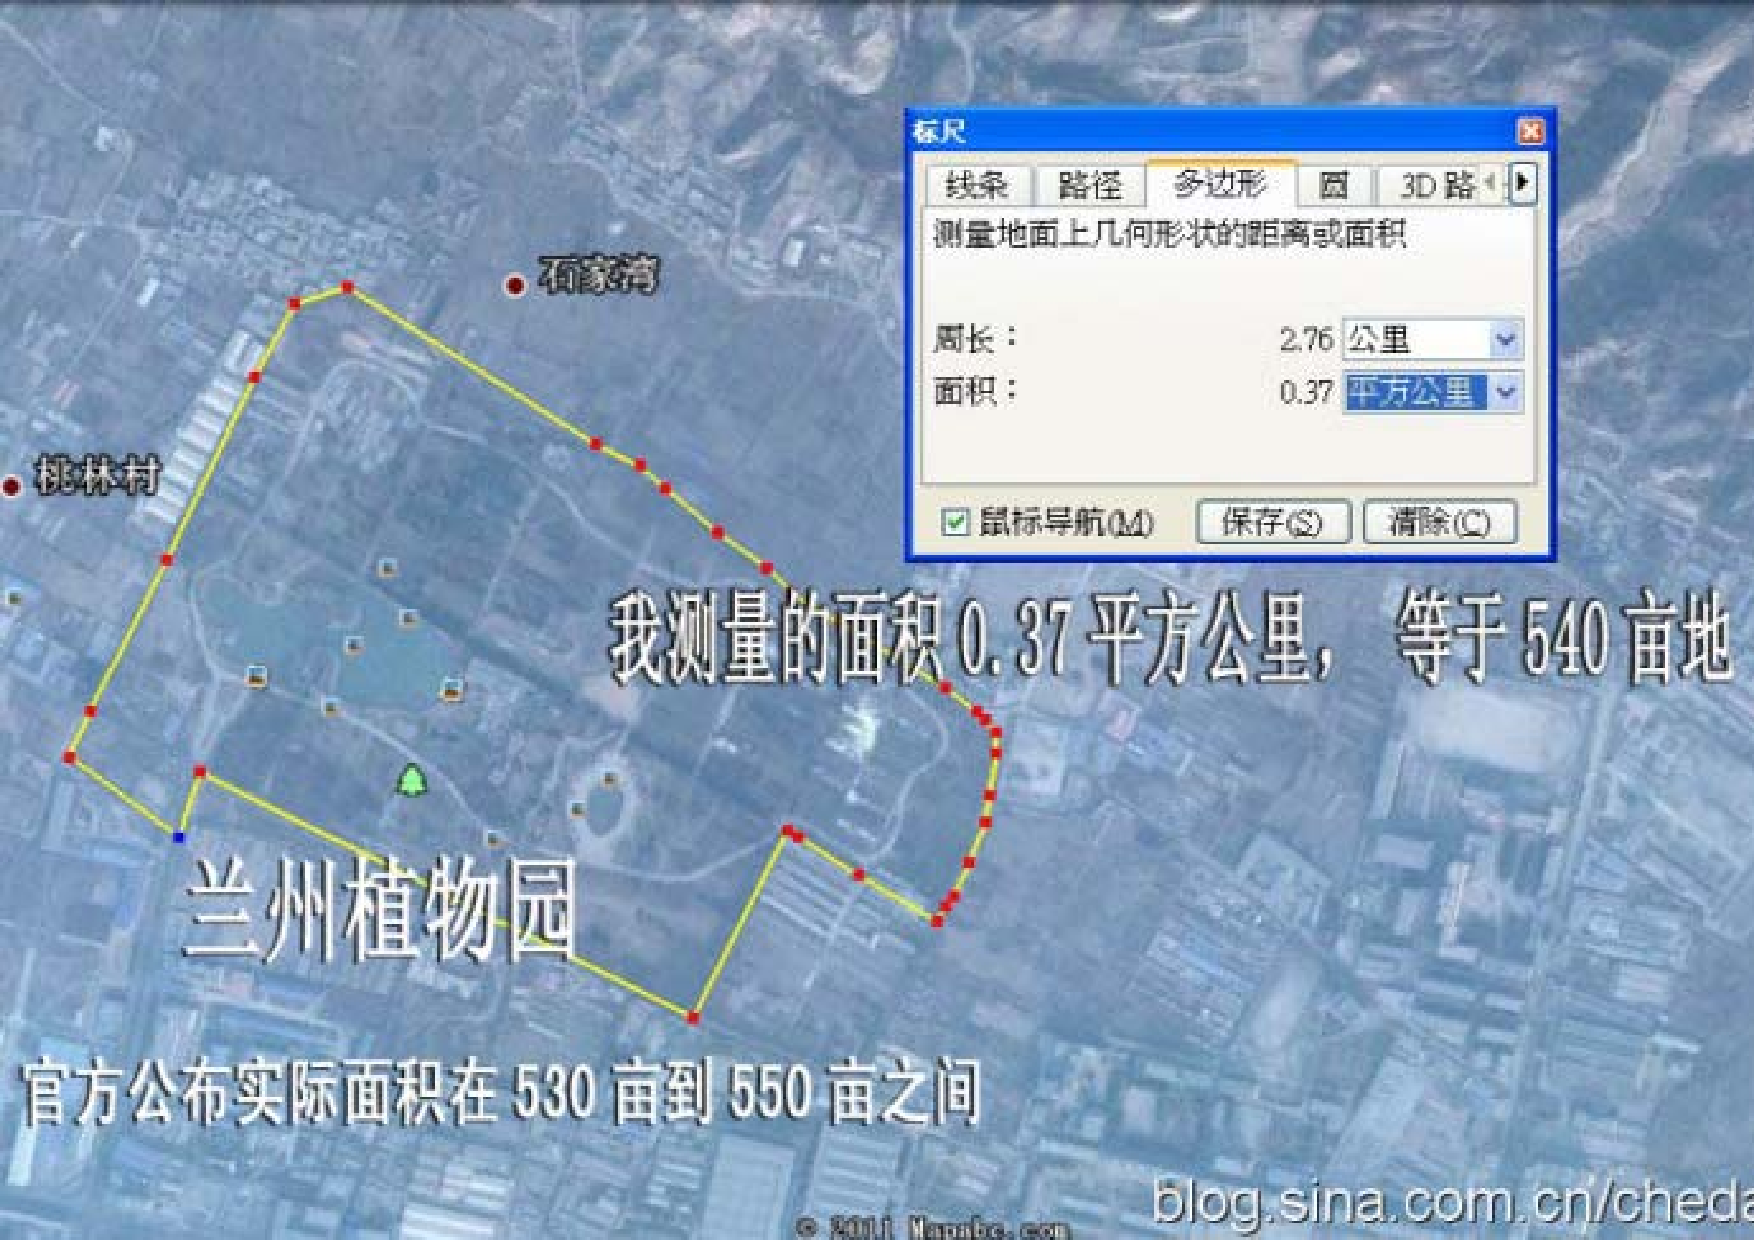
\includegraphics[width=0.7\textwidth, angle=270]{figs/4.pdf}
%%}
%\caption{地图指定区域面积计算。}
%\label{distance}
%\end{figure*}










